\documentclass[a4paper,12pt]{article}
\setlength{\parskip}{1em}
\setlength{\parindent}{0em}
\usepackage{url}
\usepackage{graphicx}
\usepackage{caption}
\usepackage[labelfont=bf, font={small}
]{caption}
\usepackage{float}
\usepackage{subcaption}

\begin{document}

\title{A Report on the Implementation and Performance of a Work Stealing Loop Scheduling Algorithm in OpenMP}
\author{Exam No. B024703}
\date{\today}
\maketitle

\section{Introduction}

This report details experiments undertaken to implement a work stealing algorithm in OpenMP. The algorithm, known as affinity scheduling, assigns work by giving blocks of work to each thread but allowing threads that have completed their block to take work from another.

The subject of this experiment was a code that contained two loops, with iterations spread evenly across threads. The author then refactored this code to use an affinity scheduling algorithm. Suboptimal parallelisation of a loop can occur when a thread finishes work that it has been assigned and must remain idle until others have completed. Affinity scheduling is a strategy for minimising this idle time. As part of the experiment, this scheduling technique was compared with the scheduling options that are defined in the OpenMP standard. The work sharing strategies defined by the standard that achieved the best results on this code were determined by a previous experiment. It is these best schedules that are used for comparison in this report.

\section{Methods}
\subsection{Compiling and Running the Original Code}
As a precaution, to check the correctness of any subsequent version, the original code was compiled in its original form. This form could be thought of as an explicitly implemented version of the static loop scheduling option in OpenMP, with the iterations of the loops evenly divided between threads.
This compilation was done using the Intel C Compiler with the \verb|-O3| option specified at compile time for maximum serial optimisation. Beyond using this to verify the correctness of any future solution and that performance was credible, analysis of the performance of this code falls outside the scope of this report.

\subsection{The Algorithm}

Each thread is initially assigned an equal amount of contiguous iterations. Where the number of iterations does not evenly divide between threads, each thread is given $ceil(n/p)$, where n is the total number of iterations and p is the total number of threads, apart from the final thread, which gets a smaller block such that the total number of iterations divided between threads is correct. 

Every thread then executes blocks of iterations whose size is $ceil(1/p)$ of the remaining iterations its local set. This continues until there are no more iterations left in the set of iterations it was initially assigned.

When a thread reaches this point it then scans the other threads to see which has the most remaining of its initial set and executes $ceil(1/p)$ of these.

While a thread has no more of its own initial set left, it continues perform this loop of scanning to see which thread has the most iterations remain and executing a block from this until there are no more iterations of the loop left to compute on any threads local set.

This algorithm has good theoretical potential. It allows each thread to maintain a contiguous block, which is beneficial for reasons of cache coherency, while preventing threads from idling by allowing them to steal work once they have finished this contiguous block.


\subsection{Implementation}

This algorithm is non-trivial to implement as it involves a great degree of synchronisation between threads, as well as requiring that each thread be aware of the progress of each other.

The awareness was maintained with the use of a shared variable which recorded the state of the algorithm. This was an array, \verb|remaining[]| containing the amount of iterations that had yet to be computed from each threads initial set. Each time a thread executed a block of size $n$ from a set $i$ of iterations it would decrement \verb|remaining[i]| by $n$.

In terms of synchronisation it was important not only that no two threads attempt to modify this array simultaneously, but that no thread attempts to modify it while another is scanning to see which thread has the most iterations remaining. To prevent these clashes a critical region was used. According to the OpenMP standard,  only one thread may enter this region at a time. This, however, can have negative effects on performance, particularly in highly parallel cases, as no thread can perform work while another is being assigned work.

To go into more technical detail, the work assignment was lifted into a function. This function takes as input an array of the amount of remaining iterations, an array of the end index of each local set (this could theoretically be derived each time but this would be less performant), the thread id of the thread requesting work and the total number of threads. It gives as an output values \verb|hi| and \verb|lo|, between which is the contiguous block of iterations that the thread should execute. The function also has a return value which it sets to true when it determines all work is complete.

The function works by first checking \verb|remaining[my_id]| to see if there is any more work in the calling threads local set. If there is then it assigns a local variable \verb|steal_id| to be equal to the threads own id. Otherwise, the thread scans the \verb|remaining| array to find the highest value, and sets steal

\section{Results}
\subsection{Correctness}
For almost all HPC applications correctness is the primary concern. The code provided included a check sum that could be used to verify the correctness of the affinity results. In all cases this sum yielded the same result as the code provided. We can therefore disregard correctness as a factor when comparing the different schedules. 

\begin{figure}
\centering
\includegraphics[width=1\textwidth]{"graphs/loop1_speeds"}
\caption{\small Graph showing execution time for loop 1 against number of threads for the affinity and dynamic, 32 schedules. Note the performance is extremely similar. }
\label{loop1scheds}
\end{figure}



\subsection{Results of Schedules on 4 Threads}
The first results gathered were execution times for each loop for every available loop schedule. The results for these are shown in Figures \ref{loop1scheds} and \ref{loop2scheds}. 

\begin{figure}
\centering
\includegraphics[width=1\textwidth]{"graphs/loop2_speeds"}
\caption{\small Graph showing execution time for loop 2 against number of threads for the affinity, dynamic, 8 and dynamic, 16 schedules.}
\label{loop2scheds}
\end{figure}

It is possible to use the results from the \verb|static| schedule to give a good experimental indication as to how evenly computational complexity is spread between iterations for the two loops. As the iterations are evenly distributed between threads with this \verb|static| method, how performant this strategy is gives a good indication as to the spread of operations between iterations. Doing this we see that for loop 1 computational complexity is far better distributed between loop iterations than in loop 2. We also see, comparing the results for \verb|static| and \verb|static,n| (see Figure \ref{loop2scheds} and Appendix A) that performance is drastically improved when these dense iterations are striped across threads. This ties in with static analysis of the code which shows that the number of floating point operations in each iteration of loop 2 is proportional to the index of the iteration.

The loop 1 results are shown in Figure \ref{loop1scheds}. These show there was a large standard deviation in all the schedules and chunk sizes. This shows a wide performance variability for this loop, particularly where the \verb|static| schedule was used. The loop 2 results shown in Figure \ref{loop2scheds} demonstrate much less performance variability for this loop, with error bars showing a much smaller standard deviation. This could be explained by the short execution time for 1000 repetitions of loop 1. This execution time is less than a second, at which point noise from I/O and other system processes can make results less reliable. 

The highest performing schedule for loop 1 was found to be \verb|dynamic,32|. This had the lowest mean execution time and also had one of the lowest standard deviations, meaning this schedule had reliably good performance for this loop.

For loop 2 we saw a general pattern where there was an optimal chunksize that was not so small that the overhead of work allocation became dominant, but not so large that the slowest chunk to complete was the dominant factor. This pattern was not followed by the \verb|guided| schedule, which performed uniformly, and relatively badly, regardless of chunksize. This may be because this scheme starts by assigning large chunks from the work queue, meaning that a large slow chunk was the dominant factor for all chunksizes.

The highest performing schedule for loop 2 was not immediately obvious. The mean execution time with the \verb|dynamic,8| and \verb|dynamic,16| was similar to the order of nanoseconds - well beyond the accuracies of this experiment. It was therefore decided that both of these schedules would be jointly selected as the best.

\subsection{Speed Up of Best Schedules}

\begin{figure}
  \centering
  
\includegraphics[width=1\linewidth]{graphs/speedup_dynamic32_loop1}
  \caption{\small Speed Up of loop 1 for the dynamic 32 schedule. A theoretical ideal speed up is shown as a black dotted line.}
  \label{dynamic32}
\end{figure}

\begin{figure}
  \centering
  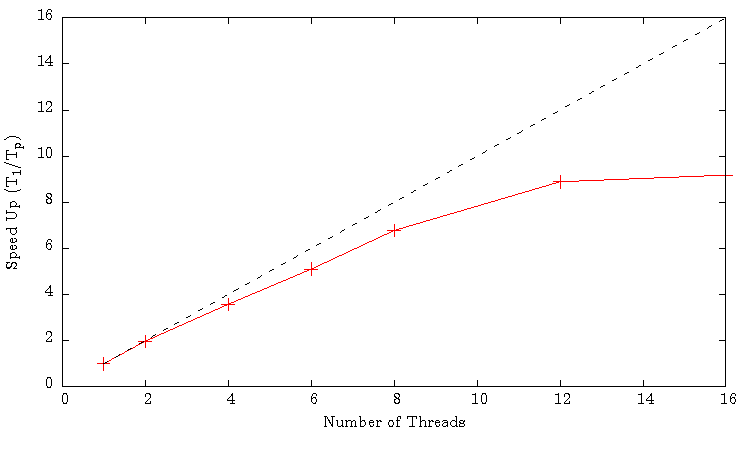
\includegraphics[width=1\linewidth]{graphs/speedup_affinity_loop1}
  \caption{\small Speed Up of loop 1 for the affinity schedule. A theoretical ideal speed up is shown as a black dotted line.}
\label{dynamic16}
\end{figure}

\begin{figure}
  \centering
  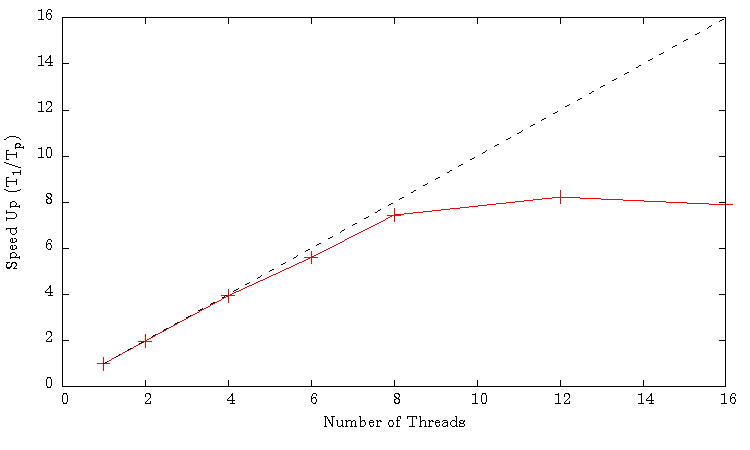
\includegraphics[width=1\linewidth]{graphs/speedup_dynamic8_loop2}
  \caption{\small Speed Up of loop 2 for the dynamic 8 schedule. A theoretical ideal speed up is shown as a black dotted line.}
  \label{dynamic8}
\end{figure}

\begin{figure}
  \centering
  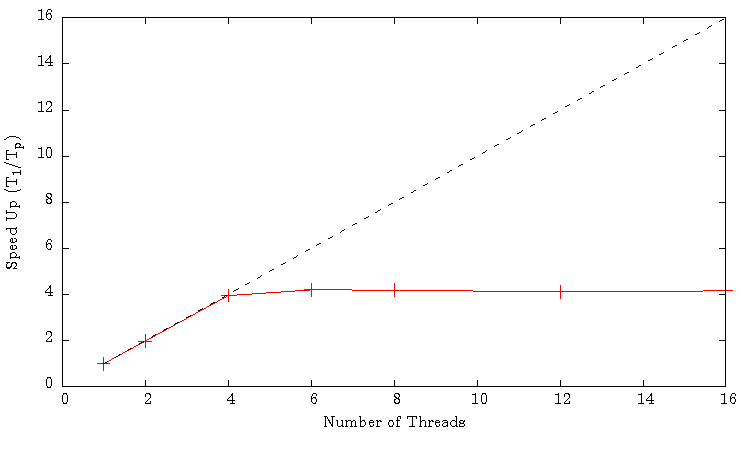
\includegraphics[width=1\linewidth]{graphs/speedup_dynamic16_loop2}
  \caption{\small Speed Up of loop 2 for the dynamic 16 schedule. A theoretical ideal speed up is shown as a black dotted line.}
\label{dynamic16}
\end{figure}


After the best schedules for loop 1 and loop 2 had been found they were then run again on 1, 2, 4, 6, 8, 12 and 16 threads. The speed up for loop  1 on the \verb|dynamic,32| schedule is shown in Figure \ref{dynamic32}. Here relatively good scalability is shown until the system reaches 12 cores. At this point no more speed up is achieved. There are many reasons that could explain this, but as the chunksize is larger for this schedule it could be that there are not enough blocks in the work queue to distribute between these threads. However, considering the results for loop 2, detailed below, it seems likely that performance is limited by the time taken for the slowest chunk of 32 to execute.

The best schedule for loop 2 was taken to be either \verb|dynamic,8| or \verb|16|. Here Figures \ref{dynamic8} and \ref{dynamic16} show extremely interesting results. The scalability completely plateaus after 8 threads where the chunksize is 8, and 4 threads where the chunksize is 16. There are two plausible explanations for this. It could be that with the larger chunksizes there is a shortage of work in the work queue for these extra threads to do, as the total work is divided into fewer larger blocks. However, because this threshold is not reached by loop 1 where the loop is split into chunks of size 32,  it seems more likely that that this is due to the time it takes for the slowest block to complete. As loop 2 is an inherently badly load balanced problem - the amount of flops per cycle is proportional to the loop index - it seems more likely that one of the threads is left with a larger block of these longer computations where the chunksize is bigger. However well distributed the remainder of the problem is, the loop cannot complete before this longest problem is solved. What we see, then, is the size of this most computationally dense chunk doubling as the chunksize doubles, leaving no further room for improvement however many threads are used.

Comparing these two loops we can see that in a more evenly distributed loop a larger chunksize is better. This is explained by reducing the overhead from each thread going to the work queue. This becomes the dominant factor where the time taken for each chunk to complete is approximately even.



\section{conclusion}
To conclude, the results found in this experiment shows that loop schedules deserve considerable attention from a programmer trying to achieve high performance with an OpenMP code. A poor selection was shown to increase execution time in some cases by more than a factor of 2 even on 4 threads and drastically reduce horizontal scalability. 

The results also demonstrate there are a balance of factors to consider when selecting the the optimal schedule. The experiments showed that the assignment of work from a queue has an overhead. It was also shown that performance could be limited by poor load balancing where a chunksize that was too large was selected, particularly where a larger number of threads are used.

Specifically in this case, results showed that the optimal scheduling strategy was for \verb|dynamic,32| for loop 1 and \verb|dynamic,8| for loop 2.

More generally it was shown that the optimal schedule will depend on the number of threads that the program will be run on as well as the nature of the loop being parallelised. It would therefore be advisable for any HPC programmer to conduct some experiments for their specific use cases before running a large job.



\bibliographystyle{plain}
\begin{thebibliography}{}
\bibitem{intelmp}
Intel Corp.
\textit{OpenMP Loop Scheduling}
\url{https://software.intel.com/en-us/articles/openmp-loop-scheduling}
Accessed: 26-10-2016

\end{thebibliography}

\pagebreak
\pagebreak
\appendix
\section{Full Results}

\begin {table}[H]
\caption {Loop 1}
\small
\center
\begin{tabular}{ | l | l | l | l | }
\hline
Schedule &  No. Threads &  Mean Time (s) &  Std. Deviation (s) \\ \hline
dynamic,32 & 1 & 1.64 & 0.00 \\ 
dynamic,32 & 2 & 0.83 & 0.00 \\ 
dynamic,32 & 4 & 0.43 & 0.01 \\ 
dynamic,32 & 6 & 0.30 & 0.01 \\ 
dynamic,32 & 8 & 0.23 & 0.01 \\ 
dynamic,32 & 12 & 0.16 & 0.01 \\ 
dynamic,32 & 16 & 0.13 & 0.01 \\
affinity & 1 & 1.65 & 0.00 \\
affinity & 2 & 0.83 & 0.00 \\
affinity & 4 & 0.46 & 0.00 \\
affinity & 6 & 0.32 & 0.03 \\
affinity & 8 & 0.24 & 0.01 \\
affinity & 12 & 0.19 & 0.01 \\
affinity & 16 & 0.18 & 0.01 \\ \hline
\end{tabular}
\end{table}



\begin {table}
\caption {Loop 2}
\small
\center
\begin{tabular}{ | l | l | l | l | }
\hline
Schedule &  No. Threads &  Mean Time (s) &  Std. Deviation (s) \\ \hline 
dynamic,8 & 1& 8.84 & 0.01\\
dynamic,8 & 2& 4.47 & 0.02\\
dynamic,8 & 4 & 2.24 & 0.01\\
dynamic,8 & 6 & 1.57 & 0.00\\
dynamic,8 & 8 & 1.18 & 0.00\\
dynamic,8 & 12 & 1.07 & 0.01\\
dynamic,8 & 16 & 1.12 & 0.10\\
dynamic,16 & 1 & 8.84 & 0.00\\
dynamic,16 & 2 & 4.47 & 0.02\\
dynamic,16 & 4 & 2.23 & 0.01\\
dynamic,16 & 6 & 2.10 & 0.01\\
dynamic,16 & 8 & 2.10 & 0.01\\
dynamic,16 & 12 & 2.15 & 0.09\\
dynamic,16 & 16 & 2.12 & 0.04 \\ 
affinity & 1 & 1.65 & 0.00 \\
affinity & 2 & 0.83 & 0.00 \\
affinity & 4 & 0.46 & 0.01 \\
affinity & 6 & 0.32 & 0.03 \\
affinity & 8 & 0.24 & 0.01 \\
affinity & 12 & 0.19 & 0.01 \\
affinity & 16 & 0.18 & 0.01 \\ \hline
\end{tabular}
\end{table}

\pagebreak
\section{Code Snippet}
\begin{verbatim}
int get_work(int *remaining, int *end_index, int myid, int nthreads, int *lo,
             int *hi)
{
  int i, chunk_size, steal_index, temp_max;
  temp_max = 1;
  // if a thread has no more work it should steal work.
  if (remaining[myid] == 0)
  {
    // use loop to find thread with most work remaining
    temp_max = 0;
    int i;
    for (i = 0; i < nthreads - 1; i++)
    {
      if (temp_max < remaining[i])
      {
        temp_max = remaining[i];
        steal_index = i;
      }
    }
  }
  else
  {
    steal_index = myid;
  }

  if (temp_max != 0)
  {
    chunk_size = (int)ceil((double)remaining[steal_index] / (double)nthreads);
    *lo = end_index[steal_index] - remaining[steal_index];
    *hi = *lo + chunk_size;
    remaining[steal_index] -= chunk_size;
    return 0;
  }
  else
  {
    return 1;
  }
}
\end{verbatim}


\end{document}